% Präambel
\documentclass[12pt,a4paper,oneside, 
liststotoc, 					% Tabellen- und Abbildungsverzeichnis ins Inhaltsverzeichnis
bibtotoc,						% Literaturverzeichnis ins Inhaltsverzeichnis aufnehmen
titlepage, 						% Titlepage-Umgebung statt \maketitle
headsepline, 					% horizontale Linie unter Kolumnentitel
%abstracton,					% Überschrift beim Abstract einschalten, Abstract muss dazu in {abstract}-Umgebung stehen
%DIV11,							% auskommentieren, um den Seitenspiegel zu vergrößern
BCOR6mm,						% Bindekorrektur, die den Seitenspiegel um 6mm nach rechts verschiebt,
]{scrreprt}		

% Laden verschiedener Packages
\usepackage{ucs} 				% Dokument in utf8-Codierung schreiben und speichern
\usepackage{url}
\usepackage[utf8x]{inputenc} 	% ermöglicht die direkte Eingabe von Umlauten
\usepackage[ngerman]{babel} 	% deutsche Trennungsregeln und Übersetzung der festcodierten Überschriften
\usepackage[T1]{fontenc} 		% Ausgabe aller zeichen in einer T1-Codierung (wichtig für die Ausgabe von Umlauten!)
\usepackage{graphicx}  			% Einbinden von Grafiken erlauben
\usepackage{amsmath}
\usepackage{csquotes}           % Zusatzpaket für Zitierungen (Nur optisch, nicht logisch)
%\usepackage{amsfonts}
%\usepackage{amssymb}
\usepackage{mathpazo} 			% Einstellung der verwendeten Schriftarten
\usepackage{textcomp} 			% zum Einsatz von Eurozeichen u. a. Symbolen
\usepackage{listings}			% Datstellung von Quellcode mit den Umgebungen {lstlisting}, \lstinline und \lstinputlisting
\usepackage[dvipsnames]{xcolor} % einfache Verwendung von Farben in nahezu allen Farbmodellen
\usepackage[intoc]{nomencl} 	% zur Erstellung des Abkürzungsberzeichnisses
\usepackage{fancyhdr}			% Zusatzpaket zur Gestaltung von Fuß und Kopfzeilen
\usepackage{epigraph}
\usepackage{svg}
\usepackage{tkz-kiviat}

\usepackage{xargs}
\usepackage{setspace}
\usepackage[smaller]{acronym}

\usepackage[]{algorithm2e} 		% Für die Verwendung von Pseudocode
\usepackage[]{algorithmicx}		% Anderes Pseudocode Paket zum testen

\usepackage[colorinlistoftodos,prependcaption,textsize=tiny]{todonotes}

\usepackage{hyperref}



% -------------------------------------------------------------------------------------------
%                     Persönliche Daten
% -------------------------------------------------------------------------------------------

\newcommand{\titel}{Bilderzeugende Verfahren zum Angriff einer Verkehrsschilder erkennenden KI}
\newcommand{\shellcmd}[1]{\\\indent\indent\texttt{\footnotesize\# #1}\\}
\newcommand{\untertitel}{}
\newcommand{\ausarbeitung}{Ausarbeitung}
\newcommand{\arbeit}{IT-Projekt Bericht}
\newcommand{\studiengang}{Informatik}
\newcommand{\autor}{Leonhard Applis, Peter Bauer, Andreas Porada und Florian Stöckl}
\newcommand{\autorShort}{L.Applis, P. Bauer, A. Porada, F. Stöckl}
\newcommand{\abgabeGI}{15.01.2019} %Abgabe beim Informaticup
\newcommand{\abgabeTH}{15.03.2019} %Abgabe bei der TH
\newcommand{\betreuerth}{Prof. Dr. Gallwitz}
\newcommand{\jahr}{2019}			% für Angabe im Copyright-Vermerk der Titelseite

%Einstellungen, Farben, Commands
\newcommandx{\unsure}[2][1=]{\todo[linecolor=red,backgroundcolor=red!25,bordercolor=red,#1]{#2}}
\newcommandx{\change}[2][1=]{\todo[linecolor=blue,backgroundcolor=blue!25,bordercolor=blue,#1]{#2}}
\newcommandx{\info}[2][1=]{\todo[linecolor=OliveGreen,backgroundcolor=OliveGreen!25,bordercolor=OliveGreen,#1]{#2}}
\newcommandx{\improvement}[2][1=]{\todo[linecolor=Plum,backgroundcolor=Plum!25,bordercolor=Plum,#1]{#2}}
\newcommandx{\thiswillnotshow}[2][1=]{\todo[disable,#1]{#2}}

% Default fixed font does not support bold face
\DeclareFixedFont{\ttb}{T1}{txtt}{bx}{n}{12} % for bold
\DeclareFixedFont{\ttm}{T1}{txtt}{m}{n}{12}  % for normal

%------------Colors ----------------
\definecolor{deepblue}{rgb}{0,0,0.5}
\definecolor{deepred}{rgb}{0.6,0,0}
\definecolor{deepgreen}{rgb}{0,0.5,0}

\pgfkeys{
	/kiviatgrad/simplify label/.code={
		\ifx\nv\undefined\else
		\pgfmathparse{Mod(\nv,5)}
		\ifdim\pgfmathresult pt>0pt
		\tikzset{opacity=0}
		\fi
		\fi
	}
}	
% ------------------Setting up environment for codes ---------------
% Python style for highlighting
\newcommand\pythonstyle{\lstset{
		language=Python,
		basicstyle=\ttm,
		morekeywords={access,and,break,class,continue,def,del,elif,else,except,exec,finally,for,from,global,if,import,in,is,lambda,not,or,pass,print,raise,return,try,while},
		morekeywords=[2]{abs,all,any,basestring,bin,bool,bytearray,callable,chr,classmethod,cmp,compile,complex,delattr,dict,dir,divmod,enumerate,eval,execfile,file,filter,float,format,frozenset,getattr,globals,hasattr,hash,help,hex,id,input,int,isinstance,issubclass,iter,len,list,locals,long,map,max,memoryview,min,next,object,oct,open,ord,pow,property,range,raw_input,reduce,reload,repr,reversed,round,set,setattr,slice,sorted,staticmethod,str,sum,super,tuple,type,unichr,unicode,vars,xrange,zip,apply,buffer,coerce,intern},%
		morecomment=[l]\#,%
		sensitive=true,%
		%otherkeywords={self,if,print,while,return,def},             % Add keywords here
		keywordstyle=\ttb\color{deepblue},
		emph={MyClass,__init__},          % Custom highlighting
		emphstyle=\ttb\color{deepred},    % Custom highlighting style
		stringstyle=\color{deepgreen},
		frame=tb,                         % Any extra options here
		showstringspaces=false            % 
}}

% Python environment
\lstnewenvironment{python}[1][]
{
	\pythonstyle
	\lstset{#1}
}
{}

% Python for external files
\newcommand\pythonexternal[2][]{{
		\pythonstyle
		\lstinputlisting[#1]{#2}}}


\usetikzlibrary{arrows} % define style of tkiz kiviat

% Abkürzungen
\newcommand{\ua}{\mbox{u.\,a.\ }}
\newcommand{\zB}{\mbox{z.\,B.\ }}
\newcommand{\bs}{$\backslash$}

\renewcommand{\nomname}{Abkürzungsverzeichnis}

% -------------------------------------------------------------------------------------------
% Definition der Kopf- und Fußzeilen
\lhead{}								% Kopf links
\chead{}								% Kopf mitte
\rhead{\sffamily{\leftmark}}				% Kopf rechts
\lfoot{}								% Fuß links
\cfoot{\sffamily{\thepage}}				% Fuß mitte
\rfoot{\sffamily{\autor}}				% Fuß rechts
\renewcommand{\headrulewidth}{0.4pt}	% Liniendicke Kopf
\renewcommand{\footrulewidth}{0.4pt}	% Liniendicke Fuß


\makenomenclature							% Abkürzungsverzeichnis erstellen
%\input{Inhalt/abkuerzungen}					% Datei mit Abkürzungen laden

% Definition of colors
\definecolor{lightblue}{rgb}{0.910,0.933,0.970}
\definecolor{lightred}{RGB}{247,238,232}
\definecolor{monochromeLightblue}{RGB}{165,188,222}
\definecolor{monochromeLightred}{RGB}{222,188,165}
\definecolor{kiviatOne}{RGB}{137,193,30}
\definecolor{kiviatTwo}{RGB}{20,128,120}
\definecolor{kiviatThree}{RGB}{208,108,32}
\definecolor{kiviatFour}{RGB}{168,26,104}

\newcommand\ColorBox[1]{\textcolor{#1}{\rule{2.5ex}{2.5ex}}}

% ----------------------------------- Links Styling -----------------------------------------
\hypersetup{
	%pdfborder = {0 0 0},
	bookmarks=true,         % show bookmarks bar?
	unicode=false,          % non-Latin characters in Acrobat’s bookmarks
	pdftitle={Erstellung von Irrbildern zur Überlistung einer Verkehrsschilder erkennenden KI}
	pdfauthor={Leonhard Applis, Peter Bauer, Andreas Porada und Florian Stöckl},     % author
	pdfsubject={IT-Projektarbeit},   % subject of the document
	pdfcreator={Leonhard Applis, Peter Bauer, Andreas Porada und Florian Stöckl},   % creator of the document
	pdfproducer={Leonhard Applis, Peter Bauer, Andreas Porada und Florian Stöckl}, % producer of the document
	colorlinks=true,       % false: boxed links; true: colored links
	linkcolor=blue,          % color of internal links (change box color with inkbordercolor)
	citecolor=CadetBlue,        % color of links to bibliography
	filecolor=magenta,      % color of file links
	urlcolor=cyan,           % color of external links
}

% -------------------------------------------------------------------------------------------
%                     Beginn des Dokumenteninhalts
% -------------------------------------------------------------------------------------------


\begin{document}
\setcounter{secnumdepth}{3}					% Nummerierungstiefe fürs Inhaltsverzeichnis
\setcounter{tocdepth}{3}
\sffamily									% für die Titelei serifenlose Schrift verwenden

% ------------------------------ Titelei -----------------------------------------------------

\thispagestyle{plain}
\begin{titlepage}
\enlargethispage{3.5cm}
\sffamily 								% Serifenlose Grundschrift für die Titelseite einstellen
\begin{minipage}{\textwidth}
	\vspace{-2cm}
	\noindent 
\includegraphics[scale=0.2]{Images/Logo_TH.png} \hfill
\end{minipage} 
\begin{center}

\huge{\textsc{\textbf{\titel}}}\\[1.5ex]
\Large{\textbf{\untertitel}}\\[5ex]
\LARGE{\textbf{\ausarbeitung}}\\[2ex]
\normalsize{~}\\[3ex]
\Large{Master-Studiengang \textit{\studiengang}}\\[1ex]
\normalsize{Technische Hochschule Nürnberg Georg Simon Ohm}\\[5ex]
von\\[1ex] \autor \\[12ex]

\begin{tabular}{ll}
	Abgabedatum:					& \quad \abgabeTH \\ 
	
	Gutachter der Hochschule: & \quad \betreuerth \\ 
	%[6ex]%formerly 5ex
	
\end{tabular} 

\end{center}

\end{titlepage}
%Starting Correct Spacing here...
\onehalfspacing 				% erzeugt die Titelseite
\pagenumbering{Roman}						% große, römische Seitenzahlen für Titelei
\addchap*{Eidesstattliche Erklärung}
Wir versichern hiermit, dass der \arbeit~ mit dem Thema

\emph{\titel}\\
selbständig verfasst wurde und keine anderen als die angegebenen Quellen und Hilfsmittel benutzt wurden. Die Arbeit wurde bisher keiner anderen Prüfungsbehörde vorgelegt und auch nicht veröffentlicht.


Wir versichern zudem, dass die eingereichte elektronische Fassung mit der gedruckten Fassung übereinstimmt.\\[10ex]

Nürnberg, den \today \\[4ex]


\rule[-0.2cm]{10cm}{0.5pt} \\

\textsc{\autor} \\[10ex]
 				% Einbinden der eidestattlichen Erklärung
\chapter*{Abstract} %*-Variante sorgt dafür, das Abstract nicht im Inhaltsverzeichnis auftaucht
This paper uses several scientific approaches to show how convolutional neural networks can be tricked into recognizing and correctly classifying road signs.
In the field of autonomous driving, neural networks have drastically increased the recognition rate, but they are still susceptible to errors in the face of deliberately generated false images. Even without information about the underlying architecture (so-called black box attacks), attacks by otherwise generated false images should be possible.
The presented methods \textit{Degeneration}, \textit{Saliency Maps} and \textit{Gradient Ascent} are successfully applied to generate false images for attacks on an unknown neural network with the help of an own neural network which serves as \textit{Substitute}.
An attack is considered "'successful"' if the image is recognized as a street sign with a confidence greater than 90\%, which a human observer would not recognize as such.
~\newline
~\newline
\begin{flushleft}
	\begin{tabular}{lp{11cm}}
		\textbf{title:} & Fooling a TrafficSign-AI \\
		\textbf{authors:}  & \autor \\
		
		%einkommentieren für TH Abgabe
		%\textbf{reviewer TH:} & \betreuerth \\
		%[6ex]%formerly 5ex
	\end{tabular} 
\end{flushleft}


\chapter*{Kurzfassung} 
Diese Arbeit zeigt anhand von mehreren wissenschaftlichen Ansätzen, wie Convolutional Neural Networks zur Erkennung und korrekten Klassifikation von Straßenschildern überlistet werden können.
Im Bereich des Autonomen Fahren wurden mit Neuronalen Netzen die Erkennungsrate drastisch gesteigert, allerdings sind diese immer noch fehleranfällig gegenüber gezielt erzeugten Irrbildern. Selbst ohne Informationen über die unterliegende Architektur (sog. Black-Box Angriffe), sollen Angriffe durch anderweitig erzeugte Irrbilder möglich sein.
Die vorgestellten Verfahren \textit{Degeneration}, \textit{Saliency Maps} und \textit{Gradient Ascent} werden erfolgreich angewendet, um mithilfe eines eigenen Neuronalen Netz welches als \textit{Substitute} dient, Irrbilder für Angriffe auf ein unbekanntes Neuronales Netz zu erzeugen.
Ein Angriff gilt als "'erfolgreich", wenn das Bild mit einer Konfidenz größer als 90\% als Straßenschild erkannt ist, welches ein menschlicher Betrachter nicht als solches erkennen würde.

~\newline
\begin{flushleft}
	\begin{tabular}{lp{11cm}}
		Titel:&  \titel \\ 
		Authoren:&  \autor \\
		%einkommentieren für TH Abgabe
		%Prüfer der Hochschule: &  \betreuerth \\ 
		%[6ex]%formerly 5ex	
	\end{tabular} 
\end{flushleft}   				% Einbinden des Abstracts

\tableofcontents							% Erzeugen des Inhalsverzeichnisses
\printnomenclature[2.0cm]					% Erzeugen des Abkürzungsverzeichnisses
\listoffigures 								% Erzeugen des Abbildungsverzeichnisses 
%\listoftables 								% Erzeugen des Tabellenverzeichnisses
\pagebreak
% --------------------------------------------------------------------------------------------
%                    Inhalt der Arbeit
%---------------------------------------------------------------------------------------------
\pagenumbering{arabic}						% arabische Seitenzahlen für den Hauptteil
\pagestyle{fancy}					
\rmfamily

% alle Abkürzungen, die in der Arbeit verwendet werden
\chapter*{Abkürzungsverzeichnis}
\addcontentsline{toc}{chapter}{Abkürzungsverzeichnis}
\begin{singlespace}
	
\begin{acronym}[Studienarbeit]
    \acro{DBMS}{Database Management System}
	\acro{ETL}{Extract-Transform-Load}
	\acro{KI}{Künstliche Intelligenz}
	\acro{SQL}{Structured Query Language}
	\acro{NN}{Neuronales Netz}
	\acro{DNN}{Deep Neural-Network}
	\acro{CNN}{Convolutional Neural-Network}
	\acro{GTSRB}{German Traffic Sign Recognition Benchmark}
	\acro{PPM}{Portable Pixmap Image}
	\acro{PNG}{Portable Network Graphic}
\end{acronym}

\end{singlespace}
\chapter{Einleitung}
\label{cha:Einleitung}
\setlength{\epigraphwidth}{4in}

%\section{Motivation}
Der Traum von einem autonom gelenkten Automobil ist so alt wie das Automobil selbst \cite{maurer_autonomes_2015}. Fabian Dröger schreibt dazu in seinem Beitrag "`Das automatisierte Fahren im gesellschaftswissenschaftlichen und kulturwissenschaftlichen Kontext"' in dem Sammelwerk "`Autonomes Fahren"' von Markus Maurer et al., wie die zunehmende Anzahl an Verkehrstoten in den USA zu Beginn des 20. Jahrhunderts in Verbindung mit den technischen Errungenschaften in der frühen Flugzeug- und Radiotechnik den Wunsch nach einem selbstfahrenden Automobil aufkommen ließen. Die Vision war, dass ein Automobil ähnlich wie ein Flugzeug durch einen Autopiloten in der Spur gehalten und gesteuert werden könnte. Für die Ansteuerung der mechanischen Teile setzte man auf eine Fernsteuerung mit Funk, die zu dieser Zeit im Bereich der \emph{Radioguidance} erforscht wurde.

Der aktuelle Stand der Technik zeigt, dass sich die Umsetzung dieser Vision schwieriger gestaltet, als zunächst angenommen. Anstelle einer autonomen Steuerung finden sich in heutigen Automobilen verschiedene Techniken zur Erhöhung der Fahrsicherheit und des Komforts. Beispiele sind Spurhalteassistenten, automatische Abstandshalter oder Einparkhilfen. Diese Funktionen unterstützen einen menschlichen Fahrer, ermöglichen jedoch noch kein selbstständiges Fahren.

Es wird aber weiterhin an der Entwicklung eines autonomen Fahrzeugs geforscht, wie die Vergabe von Forschungsgeldern\cite{bmbf-internetredaktion_auto_nodate} und Berichte von Automobil"-her"-stel"-lern\cite{bmw_autonomes_nodate} und der Presse\cite{efler_autonomes_2018} zeigen. Die Forschung im Bereich \ac{KI} hat mittlerweile einen Stand erreicht, der für die Automatisierung des Autos genutzt werden kann. Ein besonderer Fokus liegt hierbei auf dem Erkennen von Bilder aus der Umwelt mittels einer \ac{KI}. Im Straßenverkehr ist besonders die Erkennung von Straßenschildern von Bedeutung.


\section{Problemstellung}
Bei der Untersuchung von \acp{KI}, welche auf die Erkennung gewisser Muster mit einem Datensatz trainiert wurden, fiel auf, dass auch Muster, die für den Menschen in keinem erkennbaren Zusammenhang mit dem Trainingsmuster stehen, von der \ac{KI} mit hoher Konfidenz anerkannt werden. Das gezielte Ausnutzen dieses Fehlers wird in der Forschung als \textit{Adversarial Attack} bezeichnet \cite{DBLP:journals/corr/HuangPGDA17}.

Der Erfolg von \textit{Adversarial Attacks} liegt in der gezielten Stimulation von Gewichten, die die \ac{KI} basierend auf ihrem Trainingssatz festgelegt hat, beziehungsweise die vom Trainer definiert wurden. Auf diese Weise ist es möglich ein gewünschtes Feedback eines \acs{NN}s zu erhalten, obwohl das Muster für einen Menschen kaum oder gar nicht mit den Mustern des Trainingssatzes in Verbindung gebracht werden kann. Zum Beispiel haben erzeugte Fragmente zur Täuschung einer \ac{KI}, die für die Erkennung von Bildinhalten trainiert ist, selten etwas mit einem \textit{echten} Bild zu tun. Sie wirken eher wie Rauschen oder moderne Kunst. 

~\newline Das Problem an den präparierten Mustern einer \textit{Adversarial Attack} ist, dass ein Mensch schwer erkennen kann, ob ein derartiger Angriff auf die von ihm genutzte \ac{KI} unternommen wird. Er ordnet das manipulierte Muster nicht den relevanten Mustern zu, die seine \ac{KI} anerkennt.

Durch den steigenden Einsatz von Machine Learning in verschiedenen sensiblen Sektoren des täglichen Lebens, wie selbstfahrenden Autos, Terrorismusbekämpfung oder Betrugserkennung können Angriffe verheerende Schäden erzeugen und stellen ein lohnendes Ziel dar. Vor allem im Bereich des autonomen Fahrens, welcher aktuell geprägt ist durch eine Debatte über das \textit{Vertrauen in Technik} \cite{VertrauenTechnik}, können erfolgreiche Angriffe zu einem forschungsschädlichen Misstrauen führen und die Nutzung der Technik verhindern. 

~\newline Um gegen Adversarial Attacks vorzugehen, werden zunächst einige Bilder benötigt, die gezielt Gewichte einer \ac{KI} stimulieren und mit hoher Konfidenz anerkannt werden. Anschließend können, um das neuronale Netz zu härten, Tests durchgeführt werden und die Angriffe berücksichtigt werden. 

%Diese Irrbilder zu erzeugen stellt das Kernziel dieser Arbeit dar. 

\section{Ziel der Arbeit}
\label{sec:ZielDerArbeit}
Ziel dieser Arbeit ist es, Methoden und Herangehensweisen vorzustellen, um die Aufgabenstellung des Informaticup 2019 \todo{Hyperlink!} zu erfüllen: 

Hierbei soll ein neuronales Netz, welches sich hinter einer Webschnittstelle verbirgt und Verkehrsschilder erkennt, erfolgreich \textit{überlistet} werden - es sollen absichtlich Bilder erzeugt werden, welche für den Menschen keine Verkehrsschilder sind aber mit einer Konfidenz von über 90\% als solche erkannt werden. 

Die gefundenen Methoden sollen reproduzierbar sein und in einem Maße flexibel, um beliebig viele Irrbilder zu erzeugen. 

~\newline Der erweiterte Rahmen dieser Arbeit umfasst eine Dokumentation der Methoden sowie Verbesserungen und Schlussfolgerungen aus den Implementierungen zu ziehen. 

Ebenfalls geliefert werden alle Elemente, um die erzielten Ergebnisse zu reproduzieren und zu variieren. 

~\newline Nicht Ziel dieser Arbeit ist, einen Überblick über neuronale Netze, künstliche Intelligenz oder Bildbearbeitung zu vermitteln. 

~\newline Ebenfalls außerhalb dieser Arbeit liegt eine Auswertung, welche Bilder von einem Menschen als Verkehrsschilder erkannt werden. Die Aussagen über solche stützen sich ausschließlich auf die persönliche Einschätzung des Projektteams. 
\section{Aufbau der Arbeit}
Innerhalb dieser Arbeit werden zunächst in Kapitel \ref{cha:AnfAnalyse} Informationen über die Webschnittstelle gesammelt und aufbereitet. Die Webschnittstelle stellt eine zentrale Rahmenbedingung der vorliegenden Arbeit dar.


Im Abschnitt \ref{sec:EigenschaftenTrasi} wird hierfür zunächst der \ac{GTSRB} vorgestellt, welcher für das Training der Webschnittstelle verwendet wurde. Dieses Datenset bildet ebenfalls einen zentralen Ausgangspunkt für einige der verfolgten Ansätze.


Anschließend werden in Abschnitt \ref{sec:TrasiModell} die Eigenschaften des Modells zusammengefasst. 
Diese bestehen zum einen aus den offiziellen Angaben der Gesellschaft der Informatiker, zum anderen aus gewonnenen Erkenntnissen. Dieses Kapitel bildet die Grundlage, um die Schnittstelle einzuschätzen. 

~\newline Anschließend werden verschiedene Lösungsansätze vorgestellt, beginnend mit der \textit{Degeneration} in Kapitel \ref{cha:Degeneration}. 

Dieser Ansatz verändert iterativ ein Verkehrsschild, und behält die Änderungen bei, sollte der erzielte Score im akzeptablen Bereich liegen. Mit passender Bildveränderungen erzielen höhere Iterationen unkenntliche Ergebnisse. 

Innerhalb des Kapitels wird zunächst im Abschnitt \ref{sec:DegenerationKonzept} die Idee anhand von Pseudocode weiter erläutert und anschließend in Abschnitt  \ref{sec:DegenerationRemote} die Implementierung für die Webschnittstelle gezeigt. Die Ergebnisse liegen gesondert im Abschnitt \ref{sec:DegenerationErgebnisse} vor. 

Neben der Implementierung für die Webschnittstelle werden zum Abschluss des Kapitels in Abschnitt \ref{sec:DegenerationLokal} noch weitere Verbesserungen für eine lokale Implementierung vorgestellt, welche allerdings nicht für die Webschnittstelle tauglich waren.


~\newline Desweiteren werden in Kapitel \ref{cha:saliency} verschiedene Methoden zur Erzeugung von sog. \textit{Saliency Maps} (dt. Ausprägungskarte) vorgestellt. Unveränderte Bilder mit einer hohen Konfidenz werden ausgewählt, um die einzelnen Pixel hervorzuheben, welche für die Klassifikation den höchsten Einfluss hatten.

~\newline In Kapitel \ref{cha:gascent} wird das Verfahren des \textit{Gradient Ascent} beschrieben und evaluiert. Dabei wird mithilfe einer \textit{targeted Backpropagation} für jede Klasse ein Bild erzeugt, der die Funktion in Richtung der Zielklasse maximiert, bis die enthaltenen Merkmale eine hohe Konfidenz in der gewünschten Klasse ermöglichen.

~\newline Abschluss dieser Arbeit bildet im Kapitel \ref{cha:Schluss} ein Fazit über die gefundenen Methoden, sowie ein Ausblick auf weiterführende Arbeiten. 

\chapter{Analyse der Webschnittstelle}
\label{cha:TrasiAnalyse}
In das Kapitel kommen die Dinge die wir über die Trasi-AI wissen
\section{Eigenschaften des bereitgestellten Neuronalen Netz}
\label{sec:TrainingsDaten}




33 verschiedene aufgezeichnete klassenlabels (im vergleich GTSRB datensatz 43)

\begin{enumerate}
	\item 
	Aus der aufgabenstellung 64x64x3
	\item 
	bilder aus dem GTSRB [quelle] datensatz
	\item Gekürzte Klassen: Aus der analyse geht die Vermutung hervor, dass nur 33 Klassen unterschieden werden, keine 43 wie im orginal datensatz
	\item Softmax-Ausgabefunktion 
	\item Interpolationsfunktion (vllt mit einem Bild in 3 Interpolationsversionen und jeweiligen Score) 
	\item Overfitting bei Trainingsdaten
	\item unzuverlässigkeit bei nicht-Schildern (z.B. OhmLogo)
\end{enumerate}

\section{Transferierbarkeit von Angriffen auf ein Blackbox Modell}
\label{sec:TrasiModell}
Verwandte arbeiten bestätigen  die Transferierbarkeit von Angriffen, die auf einem "eigenen" neuronalen Netz erzeugt wurden und gegen ein unbekanntes Blackbox modell funktioniern

Einschränkungen? Probleme? Rechtfertigung der Implementation eines eigenen Modells


\section{Implementierung eines eigenen Modells zur Klassifizierung von Straßenschildern (Aphrodite)}
-beschreibung des APhrodite Modells


begründungen für die Designentscheidungen? Strategie/Vorbilder?

\todo{Leonhart}
\chapter{Technisches Konzept}
\section{Verwendete Technologien}
Die Umsetzung der Implementierung erfolgt innerhalb der webbasierten, interaktiven Entwicklungsumgebung Jupyter Notebook \footnote{https://jupyter.org/} (in der Version 5.7.4) zusammen mit der objektorientierten höheren Programmiersprache Python \footnote{https://www.python.org/} (in der Version 3.6.5).


Jupyter Notebook bietet aufgrund seiner plattformübergreifenden Einsatzmöglichkeit und Kompatibilität zu allen gängigen Webbrowsern eine hohe Flexibilität, was die Darstellung und Ausführung von Python-Code angeht. Darüber hinaus bietet Python eine hohe Verfügbarkeit von Open-Source-Repositories im Bereich Datenverarbeitung, Machine Learning und Deep Learning \ref{todo}. Die Programmiersprache wurde ferner im Rahmen der StackOverflow Befragung 2017 von den befragten Softwareentwicklern zur fünftbeliebtesten Technologie des Jahres 2017 gewählt \ref{todo}. Nicht zuletzt ist Python und die inbegriffenen umfangreichen Standardbibliotheken auf allen gängigen Plattformen, wie beispielsweise Linux, Apple MacOS und Microsoft Windows, kostenlos und in Quell- oder Binärform verfügbar \ref{todo}.


Als Paketmanager wird die frei verfügbare Anaconda Distribution in der derzeit aktuellsten Version 2018.12 gewählt, da sie eine vereinfachte Paketinstallation und -verwaltung ermöglicht. Darüber hinaus bietet Anaconda die Möglichkeit Jupyter Notebooks sowie Python und dessen verfügbare Pakete in verschiedenen Entwicklungs- und Testumgebungen isoliert voneinander zu verwalten und zu betreiben \ref{todo}. Schließlich erlaubt “Anaconda Accelerate” den programmatischen Zugriff auf numerische Softwarebibliotheken zur beschleunigten Codeausführung auf Intel Prozessoren sowie NVIDIA Grafikkarten \ref{todo}.


Zur fehlerfreien Ausführung des Codes der Implementierungen in den nachfolgenden Kapiteln muss Python in der Version 3.6.5 verwendet werden. Weiterhin bestehen Abhängigkeiten zu den Bibliotheken, welche in Tabelle \ref{tab:parameter} mit den dazugehörigen Versionen angegeben sind. Durch den Einsatz von Anaconda kann eine Environment erstellt werden, in der die passenden Versionen installiert werden.


\begin{table}
	\centering
	\begin{tabular}{|l|l|p{10.4cm}|}
		\hline 
		Name & Version & Beschreibung \\ 
		\hline\hline 
		Keras& 2.2.4  & Enthält Funktionen für Deep-Learning Anwendungen [7] \\ 
		\hline 
		Torchvision& 0.2.1 & Enthält Datensätze, Modellarchitekturen und gängige Bildtransformationsoperationen für Computer-Vision Anwendungen [8] \\ 
		\hline 
		OpenCV& 3.4.2  & Enthält Funktionen für echtzeit Computer-Vision Anwendungen [9] \\ 
		\hline 
		NumPy&  1.15.3& Enthält Funktionen zur effizienten Durchführung von Vektor- oder Matrizenberechnungen [10] \\ 
		\hline 
		Requests& 2.18.4 & Enthält Funktionen zur Vereinfachung von HTTP Requests [11] \\ 
		\hline 
		Pillow& 5.2.0 & Enthält Funktionen zum laden, modifizieren und speichern von verschiedenen Bilddateiformaten [12] \\ 
		\hline 
		Matplotlib& 2.2.3 & Enthält Funktionen zum Plotten von Graphen oder Bildern [13] \\ 
		\hline 
		SciPy& 1.1.0  & Enthält wissenschaftliche und technische Funktionen zur Datenverarbeitung [14] \\ 
		\hline 
	\end{tabular} 
	\caption{Paketabhängigkeiten der implementierten Software}
	\label{tab:parameter}
\end{table}

Um die Voraussetzungen zur benötigten Python Version respektive der erforderlichen Python-Bibliotheken zu erfüllen, muss beim ersten Öffnen des Jupyter Notebooks zum Saliency Map Verfahren beziehungsweise zum Gradient Ascent Verfahren immer zuerst der Code unter der Rubrik “Managing Anaconda Environment” ausgeführt werden. Andernfalls kann die korrekte Ausführung von weiteren Teilen des Codes in nachfolgenden Rubriken nicht gewährleistet werden.

\section{Transferierbarkeit von Adversarial Attacks}


\label{sec:TrasiModell}
Eine Herausforderung des Wettbewerbs ist der Umgang mit dem neuronalen Netz, welches getäuscht werden soll. Die Analyse der Web-Schnittstelle in Abschnitt \ref{sec:EigenschaftenTrasi} liefert keine genauen Informationen über das zugrunde liegende Modell, was deren Architektur oder weitere Eigenschaften angeht. Dennoch wurde bereits bestätigt, dass es selbst für "`Blackbox"' Modelle möglich ist, Irrbeispiele und Bilder zu erzeugen.


Papernot et al.\cite{papernot_+_2016} bestätigten, dass Täuschungen auf ein bekanntes Netz mit hoher Wahrscheinlichkeit auch auf fremden Modellen fehlklassifiziert werden, also, dass die Ergebnisse nicht nur ein zufälliges Ereignis aufgrund von Overfitting des spezifischen \acl{NN}es sind. Die Ergebnisse wurde an verschiedenen Modelltypen getestet (bspw. \ac{SVM}, \ac{DNN}) und zeigten immer eine in ihrer Ausprägung schwankende Korrelation zwischen Fehlklassifikation auf einem fremden Modell im Vergleich zu bekannten Modellen. 


Diese Ergebnisse führten zu dem Entschluss, ein eigenes neuronales Netz zu modellieren, welches als Substitute (dt. Ersatz) dient.


\section{Implementierung eines eigenen Modells zur Klassifizierung von Straßenschildern (Aphrodite)}
Für einige der nachfolgenden Umsetzungen wird ein selbst modelliertes \ac{NN} als Substitute verwendet. Das Modell wird im Projekt unter dem Namen \textit{Aphrodite} geführt. Bei dem \ac{NN} handelt es sich um ein Keras-Modell, welches mithilfe von Tensorflow für die Erkennung von Verkehrsschildern trainiert wurde. Das \ac{NN} wird für die lokale Degeneration in Kapitel \ref{cha:Degeneration} und im Saliency Maps Verfahren eingesetzt.

~\newline Das Modell \textit{Aphrodite} umfasst vier Convolutional-Layer, drei Dense-Layer und zuletzt im Ausgabelayer eine Softmax-Funktion für die 43 Klassen. Ein detaillierter Aufbau des Netzes befindet sich im Anhang\todo{Netzzusammenfassung als Tabelle in den Anhang}\todo{Link in den Anhang}.

~\newline Für das Training wurden die \ac{GTSRB}-Trainings- und Test-Daten verwendet. Diese wurden um die richtige Auflösung zu erreichen auf 64x64 interpoliert. 

Da die verwendete Interpolationsfunktion des Black-Box Modells des Wettbewerbs unbekannt ist, wurde für das Training jedes Bild mehrfach interpoliert und ebenfalls mehrfach für das Training verwendet. Für die Testdaten wurde eine zufällige Interpolationsfunktion ausgesucht. 

~\newline \textit{Aphrodite} erreicht eine Genauigkeit von 96.5\% bei der Erkennung der Trainingsdaten. Eine Übersicht über die Trainingsparameter findet sich im Repository unter /DegenerationCode/Training.py. \todo{Sollte man das anders schreiben? Oder packen wir das file in den Anhang?}

~\newline Der Name Aphrodite wurde gewählt, um dem ersten Modell (Model A) innerhalb des Projektes einen sprechenden Namen zu geben.

\chapter{Ansatz 1 : Greyboxing}
\label{Cha:GreyBoxing}
\section{Konzept}

\section{Implementierung und erste Ergebnisse}

\section{Tuning}

\subsection{Iteration 2: Bessere Trainingsdaten Multiclass}

\subsection{Iteration 3: Verbesserte Bilderstellung}

\subsection{Iteration 4: Automatisierte Parameterisierung der Bilder}

\section{Endergebnisse} 
\chapter{Degeneration}
\label{cha:Degeneration}
Innerhalb dieses Kapitels wird der Ansatz der \textit{Degeneration} vorgestellt.

Die Benennung schöpft sich aus der Nähe zu genetischen Algorithmen \cite{heistermann2013genetische}, allerdings aus einer invertierten Perspektive: Um auf unbekannte Modelle einzugehen, wird hierbei von einem korrekt erkannten Bild \textit{weggearbeitet}. Anstatt allerdings \textit{gute Gene} zu kombinieren \cite{schoneburg1994genetische}, wird wird eine Genmutation erzeugt und überprüft, ob diese den Anforderungen der Klassifizierung noch genügt. 

Zunächst wird das Konzept anhand von Pseudocode genauer erläutert. Anschließend wird die Implementierung eines Algorithmus vorgestellt, der das unbekannte \ac{NN} des Wettbewerbs verwendet. Den Abschluss dieses Kapitels bildet eine lokale Implementierung inklusive einiger Verbesserungen, welche sich aufgrund der Limitierungen des Zugriffes auf die \textit{remote-AI} des Wettbewerbs nicht angeboten haben.
\section{Konzept}
\label{sec:DegenerationKonzept}
Die grundlegende Idee des Algorithmus bezieht sich darauf, ein Urbild $i$ zu einem Abbild $\hat{i}$ zu manipulieren, welches von dem unbekannten Klassifizierungsalgorithmus weiterhin korrekt erkannt wird. Abhängig von der Stärke der Manipulation soll eine $Tiefe$ gewählt werden, ab welcher der Algorithmus beendet wird. Als Beispiele der Manipulation seien insbesondere Rauschen und Glätten genannt, allerdings auch Kantenschärfung und Veränderungen der Helligkeit und anderer Metaparameter. Mit fortschreitender Tiefe wird nahezu jedes Bild für den Menschen unkenntlich. Zusätzlich sollten allerdings weitere Parameter als Abbruchkriterien aufgenommen werden, konkret eine Anzahl an Gesamt-Iterationen der Manipulationsfunktionen und eine Abbruchbedingung, beispielsweise wenn keine weiteren Fortschritte erreicht werden.

\newpage
\paragraph{Pseudocode} ~\newline 
Folgende Parameter erwartet die (generische) Implementierung des Degeneration-Algorithmus: 
\begin{itemize}
	\item Einen Eingabewert $i$
	\item Eine Manipulations-Funktion $a : i \rightarrow \hat{i}$
	\item Eine Klassifizierungsfunktion $p : i \rightarrow \mathrm{R}$
	\item Eine gewünschte Tiefe $d$ (empfohlen, nicht notwendig)
	\item Eine Iterationszahl $its$ (empfohlen, nicht notwendig)
	\item Ein Schwellwert $t$ , um wie viel \% die Vorhersage schlechter sein darf, als das vorhergegangene Bild 
\end{itemize}
Auf einige der Punkte wird in den Anmerkungen gesondert eingegangen. ~\newline
\IncMargin{1em}
\begin{algorithm}
	\SetKwInOut{Input}{input}
	\SetKwInOut{Output}{output}
	\Input{i,a,p,d,its,t}
	\Output{$\hat{i}$, score}
	\BlankLine
	$depth  \leftarrow 0$, $loop \leftarrow0$ \;
	$s \leftarrow p(i)$\;
	$ii \leftarrow i , is \leftarrow s$ \;
	\While{$depth<d ~ || ~ loop <its$}{
		$ai \leftarrow a(i)$ \;
		$as \leftarrow p(ai)$ \;
		\If{$as >= is-t$}{
			$is \leftarrow as$\;
			$ii \leftarrow ai$\;
			depth++\;
		}
		loop ++\;
	}
	return ii,is\;
	
	\caption{Degeneration}\label{algo_degen}
\end{algorithm}\DecMargin{1em}
\newpage
\paragraph{Anmerkungen}~\newline 
Die Manipulationsfunktionen müssen genau ein Bild der Größe (x,y) erhalten, genau ein Bild der Größe (x,y) wiedergeben und (für die generischen Implementierungen) keine weiteren Parameter erhalten. Zusätzlich sollte die Manipulationsfunktion zufällige Elemente erhalten. Sollte eine einfache, idempotente Glättungsfunktion den Schwellwert nicht erfüllen, so wird niemals eine größere Tiefe erreicht.

Tiefe, Schwellwert und Manipulationsfunktion müssen aufeinander abgestimmt werden. Es gibt einige Funktionen, welche eine starke Veränderung hervorrufen, und für welche eine geringe Tiefe bereits ausreicht. Auf der anderen Seite dieses Spektrums können Funktionen, welche lediglich minimale Änderungen vornehmen, schnell große Tiefen erreichen, ohne ein merklich verändertes Bild hervorgerufen zu haben. Diese Parameter auszubalancieren obliegt dem Nutzer. Bei der Auswahl der Parameter sollte zusätzlich berechnet werden, wie groß die letztendliche Konfidenz ist, falls die maximale Tiefe erreicht wird. 

Innerhalb der Implementierungen sollte zusätzlich eine \textit{verbose}-Funktion eingebaut werden. Hiermit kann zum einen ein ergebnisloser Versuch frühzeitig erkannt werden und zusätzlich, ob der Algorithmus sich verklemmt hat. Üblicherweise kann man erkennen, wenn die Manipulationsfunktion \textit{zu stark}, beziehungsweise der Schwellwert zu niedrig gewählt ist.

\section{Implementierung Remote}
\label{sec:DegenerationRemote}
Im Rahmen des Wettbewerbs wird mit einer Rest-API gearbeitet, welche in Abschnitt \ref{sec:EigenschaftenTrasi} analysiert wird und besondere Herausforderungen mit sich bringt: 

\begin{itemize}
	\item Anfragen können fehlschlagen
	\item zwischen Anfragen muss ein Timeout liegen
	\item Mehrere Nutzer, welche die API mit dem gleichen API Key beanspruchen, blockieren sich
\end{itemize}
~\newline
Zusätzlich wird der Grundalgorithmus um die \textit{Verbose}-Funktion und eine History erweitert. Mithilfe der \textit{History} können nach der Ausführung des Algorithmus hilfreiche Plots erstellt werden. Diese ist in dem nachfolgenden Code in Listing \ref{lst:remoteDeg} nicht enthalten.
 
Ebenso ist anzumerken, dass ignoriert wird, welche Klasse zuerst erzeugt wird. Solange irgendeine Klasse mit einer passenden Konfidenz gefunden wird, gilt das Ergebnis als hinreichend. Im Normalfall bleibt es allerdings bei derselben Klasse. 

Die Klassifizierungsfunktion wird innerhalb der Remote-Degeneration durch einige Hilfsfunktionen umgesetzt. Diese bereiten ein als \textit{Bytearray} vorliegendes Bild auf und senden es an das Trasi-Webinterface. Dies geschieht in der Methode \textit{Scorer.Send\_ppm\_image(img)}. In der Antwort des Trasi-Webinterfaces befindet sich ein JSON-Array mit den Scores einiger Klassen des bewerteten Bildes. 

Die Hilfsmethode \textit{Scorer.get\_best\_score(response)} gibt den höchsten gefunden Score wieder.
\newpage
\begin{scriptsize}
\pythonexternal[caption=Quellcode der Remote Degeneration, label=lst:remoteDeg]{CodeSnippets/remoteDegenerationSnippet.py}
\end{scriptsize}
\newpage
\section{Ergebnisse Remote}
\label{sec:DegenerationErgebnisse}
In diesem Abschnitt werden die mit der Degeneration erzielten Ergebnisse in Bezug auf die Trasi-Schnittstelle vorgestellt. Zunächst werden einige positive Beispiele (Erfolge) gezeigt, anschließend wir auf einige Probleme, die aufgetreten sind, eingegangen und zuletzt wird ein kurzes Zwischenfazit gezogen. 
\paragraph{Positive Ergebnisse} ~\newline Die zuverlässigsten Ergebnisse werden mit einfachem Rauschen erzeugt. Die Abbildung \ref{fig:stoptiefe600} zeigt, dass zunächst vorallem die Pixel außerhalb des eigentlichen Schildes verändert werden. Dieses Verhalten wird erwartet. Die farbstarken bunten Pixel sind hierbei entstanden, da Werte welche die gültige Reichweite [0,255] verlassen, wieder zyklisch zurück in den Farbbereich geholt werden. Sollte ein Farbwert durch das Rauschen einen Wert -2 erreichen, wird er auf 253 gesetzt.  

\begin{figure}[h]
	\centering
	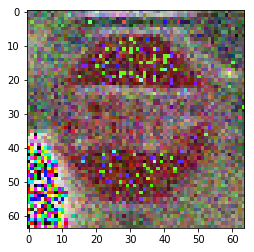
\includegraphics[width=0.4\linewidth]{Images/DegenSamples/StopTiefe600}
	\caption[Degeneration Tiefe 600]{Rausch - Degeneration mit 600 Iterationen}
	\label{fig:stoptiefe600}
\end{figure}

Während die Abbildung \ref{fig:stoptiefe600} noch als Verkehrsschild zu erkennen ist, führt ein längeres Ausführen der Degeneration zu einem Ergebnis wie in Abbildung \ref{fig:stoptiefe4000}. Um dieses Ergebnis zu erzielen wurden 4400 Sekunden benötigt, also ca. 73 Minuten.

\begin{figure}[h]
	\centering
	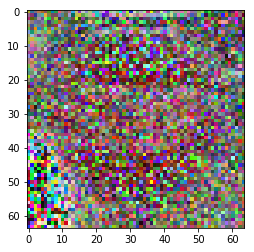
\includegraphics[width=0.4\linewidth]{Images/DegenSamples/StopTiefe4000}
	\caption[Degeneration Tiefe 4000]{Rausch - Degeneration mit 4000 Iterationen}
	\label{fig:stoptiefe4000}
\end{figure}

Die Plots in Abbildung \ref{fig:plotTiefe4000} stellen den Verlauf des Algorithmus dar: Das erste Diagramm zeigt einen Verlauf der aktuellen \textit{Tiefe} über die Iterationen, der zweite die jeweils produzierte Genauigkeit der jeweiligen Iteration (nicht nur die der akzeptierten), und der letzte Plot visualisiert diejenigen Iterationen, an welchen eine Änderung stattgefunden hat (weißer Strich) oder keine (schwarzer Strich). Innerhalb der Implementierung werden ebenfalls standartmäßig diese Plots erzeugt.

\begin{figure}[h]
	\centering
	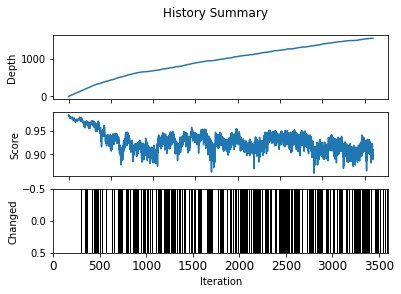
\includegraphics[width=0.6\linewidth]{Images/DegenSamples/StopTiefe4000Plot}
	\caption[Plot Degeneration]{Plot der Rausch-Degeneration}
	\label{fig:plotTiefe4000}
\end{figure}
~\newline Es wurden ebenfalls einige sehr positive Ergebnisse mit einer Mischung aus starkem Rauschen und Glätten erzeugt. Allerdings waren diese nicht zuverlässig reproduzierbar. 

\paragraph{Negative Ergebnisse} ~\newline Es gibt zwei primäre Fehlerquellen in Bezug auf die Remote-Degeneration: Die Auswahl von Bildern, welche im GTSRB-\textit{Training}-Set waren, sowie die Auswahl ungeeigneter Manipulationsfunktionen. 
~\newline
Das \ac{NN} des Wettbewerbs scheint sich die Bilder aus dem Trainingsset \textit{gemerkt} zu haben. Bereits minimale, unwichtige Änderungen des Schildes (z.B. Einfügen einiger blauer Punkte im Hintergrund) führen zu einer drastischen Verschlechterung des Ergebnisses. Dieses starke \textit{Ausschlagen} des Scores macht die Benutzung der Degeneration unbrauchbar.
\begin{figure}[h]
	\centering
	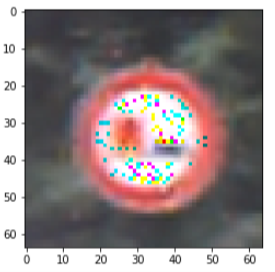
\includegraphics[width=0.5\linewidth]{Images/DegenSamples/OverFitSmaller}
	\caption[Degeneration overfit]{Rausch-Degeneration auf Trainingsbild - 36000 Iterationen}
	\label{fig:DegenOverfit}
\end{figure}
~\newline
Dieses Problem hat sich herauskristallisiert, als über einen längeren Zeitraum (\textasciitilde  10 Stunden) kein Bild erzeugt wurde, welches auch nur leicht verändert wurde. Die einzigen Änderungen, welche erzielt werden, befinden sich innerhalb des weißen Bereiches des Überholverbotsschildes, wie in Abbildung \ref{fig:DegenOverfit}. Es werden aber keine Änderungen außerhalb des Schildes vorgenommen, wo diese zu erwarten wären und bei vorhergehenden Versuchen auch zu beobachten sind (vgl. Abbildung \ref{fig:stoptiefe600}). 
~\newline
Dieses Problem tritt ausschließlich, allerdings zuverlässig, bei der Verwendung von Bildern aus dem Trainingsset auf. Es tritt nicht auf, sobald man Bilder aus dem Test-Set oder \textit{GTSRB-fremde} Bilder verwendet. Voraussetzung dabei ist, dass sie eine akzeptable Startkonfidenz besitzen. 

Innerhalb der lokalen Implementierung ist dieses Problem ebenfalls aufgetreten, konnte allerdings behoben werden, sobald man das Overfitting erkannt hatte.
\paragraph{Fazit} ~\newline
Innerhalb dieses kurzen Zwischenfazits sollen noch einmal die Vor- und Nachteile der Degeneration zusammengefasst werden:
\begin{table}[h]
	\centering
\begin{tabular}{|p{7.5cm}|p{7.5cm}|}
	\hline 
	\textbf{Vorteile} & \textbf{Nachteile} \\ 
	\hline 
	\textbf{Model-Agnostic:} \newline Der Algorithmus funktioniert unabhängig und ohne Wissen über das zugrundeliegende Modell & \textbf{Zeitintensiv:} \newline v.A. die Remote-Variante benötigt größere Zeitspannen \\ 
	\hline 
	\textbf{Kontext-Unabhängig:} \newline Die Herangehensweise ist nicht auf Bilderkennungen limitiert & \textbf{Vorwissen benötigt:} \newline Das Anwendungsfeld des zugrundeliegenden Models muss bekannt sein und ein geeignetes Startbild muss ausgewählt werden  \\ 
	\hline 
	\textbf{Erweiterbar:} \newline Die Manipulationsfunktionen können weiter ausgebaut werden und haben noch großes Potenzial & Die Degeneration erzielt bei empfindlichen Modellen schlechtere Ergebnisse - gerade sorgfältig trainierte Modelle sollten lange brauchen, um so überlistet zu werden \\ 
	\hline 
	\textbf{Simpel:} \newline Der Algorithmus ist einfach implementiert und erläutert, er benötigt keine höhere Mathematik oder Vorwissen zur Thematik \textit{Machine Learning} und der Modelle/Verfahren im Speziellen & Im Remote-Umfeld kann die Degeneration als DDoS wahrgenommen werden und entsprechend frühzeitig unterbunden werden. \\ 
	\hline 
\end{tabular} 
\caption{Zwischenfazit Degeneration}
\label{tab:FazitDegeneration}
\end{table}

Als besonderen Fall sind solche Modelle zu nennen, die mit jeder Anfrage \textit{hinzulernen}: ~\newline Diese sind entweder besonders anfällig gegenüber der Degeneration, weil sie die bereits veränderten Bilder als \textit{korrekt} klassifizieren und somit den Entstehungsprozess der Degeneration verinnerlichen oder sie \textit{härten} sich mit jedem Versuch gegen die neuen Änderungen und sind de facto immun gegen diesen Angriff.  

Solche permanent trainierenden Modelle sind in der Praxis allerdings selten im Einsatz, da sie für eine Vielzahl verschiedener Angriffe anfällig sind. Als einfaches Beispiel ist der Chatbot \textit{Tay} von Microsoft zu nennen: Dieser sollte angenehme Unterhaltungen mit Twitternutzern führen und aus den enstandenen Konversationen kontinuierlich weiterentwickelt werden \cite{mstay}. Innerhalb weniger Stunden gelang es einigen böswilligen Nutzern, dass Tay rassistische Äußerungen von sich gab \cite{mstaydown}. Microsoft hat den Service von Tay am zweiten Tag eingestellt. 
\section[Implementierung Lokal]{Implementierung Lokal \newline Anpassungen und Verbesserungen}
\label{sec:DegenerationLokal}

Innerhalb dieses Abschnittes werden zunächst die Änderungen bei der lokalen Verwendung des Algorithmus kurz behandelt und anschließend zwei konzeptionelle Verbesserungen vorgestellt: Parallel- und Batch-Varianten des Algorithmus. 

Auf weitere Code-Beispiele wird im Rahmen des Umfanges verzichtet. Sie befinden sich im Anhang.

\paragraph{Anpassungen} ~\newline Für die lokale Implementierung wurde zunächst von Grund auf ein eigenes Modell mithilfe der \ac{GTSRB}-Daten trainiert (siehe dazu Abschnitt \ref{sec:ImplAphrodite}). Das \textit{Scoring} der Remote-Implementierung wird durch die \textit{predict()}-Funktion des Models ersetzt.

Als zusätzliche Erweiterung wird für die lokale Implementierung umgesetzt, dass sich der Nutzer für eine bestimmte Klasse entscheiden kann, auf welche die Degeneration ausgelegt ist. Es wird also zuverlässig bspw. ein Stoppschild erzeugt, und kein beliebiges Schild mit hohem Score. 

~\newline Des Weiteren entfällt die Wartezeit, welche zwischen Anfragen an die Schnittstelle benötigt wird. Auf diese Weise erhöht sich die Geschwindigkeit des Algorithmus maßgeblich. 

~\newline Eine zusätzliche, passive Verbesserung wird erzielt, indem die GPU-Acceleration Funktionen von Tensorflow verwendet werden. Diese beschleunigen nicht nur das Training des lokalen Models maßgeblich, sondern auch die Vorhersagen. Insbesondere die Batch-Variante konnte im Zusammenhang mit der eingesetzten NVIDIA Grafikkarte GTX 1070\footnote{https://www.nvidia.com/en-gb/geforce/products/10series/geforce-gtx-1070/} um den Faktor 20 beschleunigt werden.


\paragraph{Fazit}~\newline Das wichtigste Fazit, welches im Umgang mit der lokalen Implementierung gezogen werden kann, ist die Nichtverwendbarkeit der lokalen Bilder für die Schnittstelle. Während dies ursprünglich die Motivation war, schnell lokal Bilder zur Täuschung der "`Black Box"' des \ac{GI}-Wettbewerbs zu erzeugen und remote zu verwenden, stellte sich heraus, dass die lokalen Bilder keine guten Scores an der Schnittstelle erzielten und vice versa. 

~\newline Es ist anzunehmen, dass die Modelle dieselben Stärken haben bei der korrekten Erkennung von Verkehrsschildern, allerdings unterschiedliche \textit{Schwächen}. Die erzeugten Bilder zur Täuschung scheinen im Model selbst zu fußen und sind somit hochgradig spezifisch. 

~\newline Die meisten stark veränderten Bilder, welche i.A. nicht mehr vom Menschen als Verkehrsschilder erkannt werden, erzeugen bei dem \ac{NN}, welches im Algorithmus verwendet wird, Werte >90\%, und beim anderen Modell zuverlässig einen Score von $\approx$30\%. 

Für ein Bild, welches an sich nichts mehr mit einem Verkehrsschild zu tun hat, sind dies immer noch hohe Werte und die Zuverlässigkeit mit der dieser Zusammenhang auftritt lässt einen leichten, inhaltlichen Zusammenhang der Bilder erahnen.

\newpage
\subsection{Batch-Degeneration}
Innerhalb des Batch-Variante wird anstatt eines einzelnen Bildes ein Array aus $n$ veränderten Bildern erzeugt. 

Diese werden alle bewertet und falls das beste Bild des Batches den Schwellwert erfüllt wird mit dem besten Bild weiter gearbeitet. Dieses Verfahren entspricht deutlich näher der Genoptimierung von genetischen Algorithmen \cite{gerdes2013evolutionare}: Es wird aus $n$-Genen das beste ausgewählt. 

\begin{figure}[h]
	\centering
	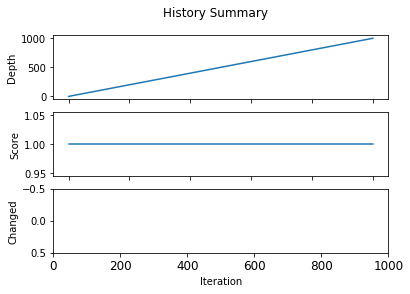
\includegraphics[width=0.5\linewidth]{Images/DegenSamples/BatchDegPlotTiefe1000}
	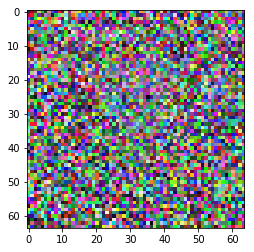
\includegraphics[width=0.35\linewidth]{Images/DegenSamples/BatchDegTiefe1000}
	\caption[Batch-Degeneration-Plot]{Verlauf der Batch-Degeneration mit Batchsize=10 und Tiefe=1000}
	\label{fig:batchdegplottiefe1000}
\end{figure}

Abbildung \ref{fig:batchdegplottiefe1000} zeigt den deutlich besseren Verlauf der Batch-Degeneration gegenüber der unveränderten Implementierung in Abbildung \ref{fig:plotTiefe4000}. Auffallend ist die durchgängige Veränderung und die gleichbleibend hohe Konfidenz von mehr als 99.9\% \footnote{Innerhalb des Plots wird es auf 1 gerundet}. 

~\newline Dieses Verhalten für die Webschnittstelle des \ac{GI}-Wettbewerbs einzusetzen ist möglich, allerdings wurde aufgrund der Wartezeit zwischen den Anfragen davon abgesehen. 

~\newline Diese Variante profitiert maßgeblich von der \textit{GPU-Acceleration} innerhalb Tensorflows. 

Selbst ohne Verwendung des CUDA-Frameworks ist ein Tensorflow-Model auf Batch-Verarbeitung ausgelegt. 

Die optimale Batchgröße zu finden ist systemabhängig und sollte kurz getestet werden. Insgesamt benötigt die Batch-Degeneration trotzdem maßgeblich mehr Zeit: Für das Beispiel in Abbildung \ref{fig:batchdegplottiefe1000} wurden ca. 15 Minuten benötigt, was knapp 5 mal so lange ist wie die ursprüngliche Implementierung. 

~\newline \textbf{Anmerkung:} Ein prinzipielles Problem der Batch-Degeneration liegt in der Zufälligkeit der Manipulationsfunktion. Als Beispiel sei einfaches Rauschen gewählt. 

Ein naheliegendes Verhalten für den Algorithmus ist von den 100 erzeugten Bildern dieses auszuwählen, welches das geringste Rauschen aufweist und als solches am wenigsten verändert wurde. Im Normalfall weist das am wenigsten veränderte Bild den nähesten Score auf. 

Glücklicherweise ist dies ein hypothetisches Problem und in der tatsächlichen Implementierung nicht aufgetreten. Dennoch sollte es vor allem für die Manipulationsfunktion berücksichtigt werden. Im Falle einer Manipulationsfunktion, welche konstante Elemente beinhaltet (zum Beispiel Glätten oder statische Veränderungen der Helligkeit) fördert die Batch-Degeneration den selektiven Ansatz.
\subsection{Parallel-Degeneration}
Die Parallel-Variante stützt sich auf die Idee, mehrere Threads zu starten, welche gleichzeitig eine Degeneration durchführen.

Sobald ein einzelner Thread die gewünschte Tiefe erreicht hat, wird der Prozess beendet. 

~\newline Die Implementierung der Parallel-Degeneration ist aufgrund mehrerer technischer Gründe gescheitert: 

\begin{itemize}
	\item Modelgröße: Jeder Thread braucht ein eigenes Model, welches allerdings zu groß war. Naive Benutzung eines gemeinsamen Models führen zu Race-Con"-ditions, \textit{geschickte} Benutzung des Models führen zu einem Verhalten wie innerhalb der Batch-Variante
	\item Numpy-Arrays: Die Bilder für die lokale Degeneration lagen als Numpy-Arrays vor, welche ein besonderes Verhalten und eine besondere Benutzung innerhalb der Parallelverarbeitung benötigen \footnote{Dieses Problem ist sicherlich lösbar lösbar, allerdings ein Problem aus dem Bereich der Parallelverarbeitung, was im Kontext dieser Arbeit nicht weiter verfolgt wird.}. 
	\item Grafikkarteneinbindung: Sobald die GPU-Acceleration innerhalb Tensorflows eingerichtet ist, werden (nahezu alle) Anfragen an die Grafikkarte weitergeleitet. Diese unterstützt das parallele Verhalten der einzelnen Threads nicht. 
\end{itemize} 
~\newline 
Die Probleme sind hardware- oder frameworkbezogen. Je nach Umfeld können diese somit entfallen. Race-Conditions entfallen beispielsweise, wenn man in der Cloud arbeitet.

~\newline Diese Variante war für die Remote-Implementierung nicht umsetzbar, da gleichzeitige Anfragen (mit dem selben API-Key) fehlschlagen. Ein internes Scheduling der Anfragen führt nicht zu schnelleren Ergebnissen. 
\subsection{Tree-Degeneration}
Diese Variante führt eine Merkstruktur ein, welche die bisherigen Ergebnisse und Schritte zwischenspeichert. 

~\newline Das bisherige Verhalten entspricht dem einer Liste, bei welcher lediglich der letzte Knoten verwendet wird. Mit dem jeweils letzten Bild wird weitergearbeitet, bis entweder ein neues korrektes Bild erzeugt wird oder der Algorithmus endet. 
\begin{figure}[h]
	\centering
	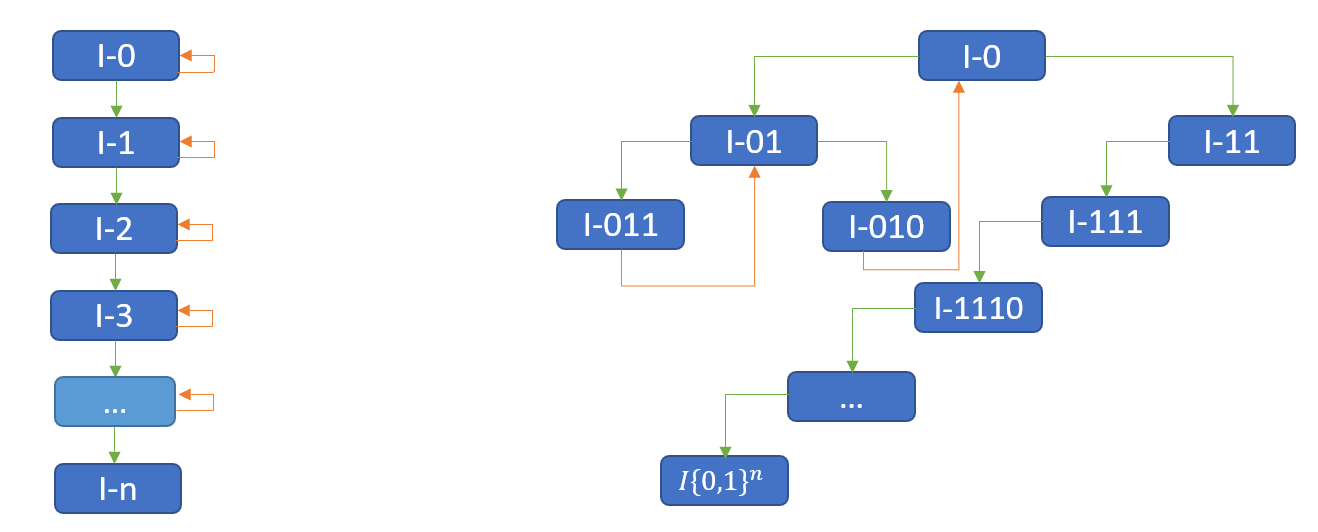
\includegraphics[width=0.8\linewidth]{Images/DegenTreeNormal}
	\caption[Tree-Degeneration]{Derzeitige Implementierung und eine Baum-basierte Implementierung}
	\label{fig:degentreenormal}
\end{figure}


~\newline Die Variation beinhaltet das führen eines \textit{Retry-Counters}, welcher bei jedem Versuch von einem Knoten erhöht wird. Sollte eine gewisse Anzahl an Versuchen ergebnislos bleiben, wird der aktuelle Knoten verworfen und der Vorgänger benutzt. 

~\newline Dieses Verhalten führt, je nach gewählter Maximalanzahl der Kinder eines Knotens, zu einem (Binär-)Baum. Das Abbruchkriterium der Tiefe kann weiterhin beibehalten werden und entspricht der Tiefe des Baumes. Im Falle eines versuchs- oder zeitbedingten Abbruchs wird das Bild mit der bisher größten Tiefe ausgegeben.

~\newline Die Entwicklung dieser Variante entstand durch die Beobachtung, dass die Geschwindigkeit der Degeneration stark abhängig sind vom Ausgangsbild. Es kann ein Bild erreicht werden, welches sehr \textit{sensibel} wahrgenommen wird und deutlich schwerer Änderungen \textit{toleriert}.

~\newline Die Batch-Degeneration ist mit dieser Variante frei kombinierbar.  
\chapter{Saliency Maps}
\label{cha:saliency}
Das Saliency Map Verfahren wurde erstmals von den Neurowissenschaftlern Itti et al. \cite{itti_model_1998} in ihrer Studie vorgeschlagen. Die Studie beschreibt eine Methode zur Extraktion von einzigartigen Merkmalen, wie beispielsweise Farben, Farbintensitäten und Strukturen, sogenannten High-Level Features, aus Bildern, die wiederum in sogenannten Saliency Maps topografisch visualisiert werden. Diese High-Level Features sind nichts anderes als spezifische Pixel im Bild auf Mikroebene (Low-Level Features), welche die optisch ansprechendsten respektive bedeutendsten Stellen in einem Bild repräsentieren. 

Um also spezifischen Bildmerkmalen eine semantische Bedeutung zuzuordnen, werden beispielsweise Farbbilder anhand des Saliency Map Verfahrens in Schwarzweißbilder umgewandelt, um die stärksten darin vorhandenen Farben zu analysieren und zu extrahieren.

\section{Konzept}
Bei \ac{CNN} werden Merkmale von Eingabebildern extrahiert, indem zunächst im Input-Layer Low-Level Features und mit jeder weiteren Schicht des Netzwerks immer komplexere Merkmale (High-Level Features), wie etwa Kanten, Rundungen oder Strukturen erlernt werden \cite{stanford_unsupervised_tutorial}.

Diese Kenntnis um \ac{CNN} und Saliency Maps machten sich Simonyan et. al erstmalig im Kontext von Deep Learning zunutze, um die gelernten Merkmale des zugrunde liegenden \ac{CNN} anhand von Saliency Maps zu visualisieren \cite{simonyan_deep_2013}. 
Die in der Arbeit von Simonyan et. al erzeugten Bilder sind hierbei nicht oder nur ansatzweise für den Menschen erkennbar, wurden jedoch vom zugrunde liegenden \ac{CNN} mit einer hohen Konfidenz richtig klassifiziert werden.


Aus dieser Kenntnis ergeben sich folgende Hypothesen:
\begin{itemize}
	\item Ein Convolutional Neural Network mit beliebiger Architektur, jedoch trainiert mit demselben Datensatz (\ac{GTSRB}) wie das Black Box Modell (aus der Aufgabenstellung), lässt sich ähnlich gut angreifen wie das Black Box Modell selbst.
	\item 	Saliency Maps repräsentieren die wesentlichen Merkmale, die das Convolutional Neural Network zu den Eingabebildern gelernt hat. Die erzeugten Bilder mit dem Saliency Map Verfahren werden wiederum vom \ac{CNN} mit einer hohen Konfidenz richtig klassifiziert, das heißt das jeweils erzeugte Bild wird vom \ac{CNN} als Verkehrszeichen erkannt und mit hoher Konfidenz richtig klassifiziert, ist jedoch für den Menschen nicht als solches erkennbar.
\end{itemize}

%Ein verbreitetes Verfahren aus dem Bereich Computer Vision zur Visualisierung relevanter Pixel ist die Erstellung von \textit{Saliency Maps} (dt. Ausprägungskarten). Diese können verwendet werden, um die Qualität, sprich Aussagekraft, jedes einzelnen Bildpunkts ersichtlich zu machen. Simonyan et al. \cite{simonyan_deep_2013} führt die grundlegende Methodik entsprechend Saliency Maps weiter aus und unterscheidet zwischen einer allgemeinen “'Klassen-Definierenden”' Saliency Map sowie einer Saliency Map zu einem gegebenen Eingabebild entsprechend der Zielklassen.
%
%
%Gebräuchliche Anwendung dieses Verfahrens im Machine Learning Bereiches betreffen der Darstellung von High Level Features einzelner Neuronen \cite{liu_delving_2016} im Bezug auf eine gezielte Klasse. Diesen Ansatz weiterverfolgend, entsprechen die erzeugten Saliency Maps im letzten Layer einer starken Neuronenaktivierung, die einer "'High Level”' Darstellung der gezielten Klasse entspricht, die vom \ac{NN} für das Bild errechnet wurde. 
%
%
%Diese Saliency Map sollte also im Rückschluss mit einer hohen Konfidenz bezüglich der entsprechenden Klasse klassifiziert werden, wenn das erzeugte Bild als Eingabe verwendet wird. Daraus ergibt sich die Hypothese, mit Hilfe dieser Visualisierung für den Menschen semantisch nicht erkennbare Verkehrszeichen Bilder zu erzeugen, die hohe Zielkonfidenzen von 0.9 oder mehr erreichen. Die beschriebene Methode wird in der Implementierung als “'Vanilla Saliency”' bezeichnet.


\section{Implementierung}

Als vorverarbeitenden Schritt werden zunächst alle 12.630 Bilder aus dem GTSRB-Testdatensatz, welche in 24-Bit Farbtiefe und im \ac{PPM} Dateiformat vorliegen, in das \ac{PNG} Dateiformat konvertiert und im Dateisystem abgespeichert.


Ein eigenes \ac{CNN} Modell („Aphrodite“) wird mit dem \ac{GTSRB}-Datensatz trainiert.

Die  vorliegenden \ac{PNG}-Bilder werden anhand dem „Aphrodite“-Modell klassifiziert:
Nur diejenigen Bilder, welche vom „Aphrodite“-Modell mit einer Konfidenz von 100\% korrekt klassifiziert wurden (3.063/12.630) werden im Dateisystem in einem eigenständigen Verzeichnis abgespeichert.


Gemäß einer auf die Anforderungen an die Aufgabenstellung abgewandelten Variante zu Anh \cite{anh_implementations_2019}, erfolgt nun die Implementierung der verschiedenen Saliency Map Verfahren.


Hierzu werden zunächst die drei Basismethoden „Vanilla“ \cite{simonyan_deep_2013}, „Guided Backpropagation“ \cite{springenberg_striving_2014} und „Integrated Gradient“ \cite{sundararajan_axiomatic_2017} implementiert. 
Unter Hinzufügung von Zufallsrauschen, gemäß \cite{smilkov_smoothgrad:_2017}, werden die Basismethoden verbessert, wie die Gegenüberstellung der Ergebnisse zu den eingesetzten Verfahren in Kapitel \ref{sec:SalErgebnisse} verdeutlicht.
Diese optimierten Varianten werden als „Smoothed Vanilla“, „Smoothed Guided Backpropagation“ und „Smoothed Integrated Gradient“ bezeichnet und implementiert.


Jedes der Saliency Map Verfahren wird auf die in Schritt 3 erzeugten Bilder angewendet. Diese Bilder werden nacheinander vom Dateisystem geladen und anschließend auf eine Zielbildgröße von 64 x 64 Pixel skaliert. 
Zur Extraktion und Visualisierung der gelernten Merkmale des zugrunde liegenden Modells (Aphrodite) zu jedem skalierten Eingabebild, wird das gewählte Saliency Map Verfahren auf jedes Eingabebild, unter Verwendung des trainierten „Aphrodite“-Modells, angewendet. 
Die damit erzeugten Bilder werden anschließend in einem nach dem verwendeten Saliency Map Verfahren bezeichneten Verzeichnis in der Größe 64 x 64 Pixel im Dateisystem abgespeichert.


Zur abschließenden Evaluierung der erzeugten Bilder am Black Box Modell, werden alle Bilder zu jedem eingesetzten Saliency Map Verfahren im Zyklus von 60 Bilder pro Minute (Übertragungslimit pro Minute an der Remote-Webschnittstelle) an das Trasi-Webinterface gesendet. Die Informationen, das heißt die vom Black Box Modell erkannte Zielklasse und Konfidenz, werden anschließend aus dem HTTP-Responsecode zu jedem übermittelten Bild in zwei verschiedenen Logdateien gespeichert: Die erste Logdatei speichert alle Ergebnisse aus dem jeweiligen HTTP-Responsecode, wohingegen die zweite Logdatei nur gefilterte Ergebnisse, das heißt Konfidenzen von mehr als 90\%, zu den übermittelten Bildern enthält.


%
%Nachfolgend wird der vollständige Datensatz lokal am eigenen Modell klassifiziert und alle Bilder mit einer Konfidenz von 100\% separat gesammelt. 
%
%Die vorgestellten Verfahren Vanilla Saliency\cite{simonyan_deep_2013}, Guided Backpropagation\cite{springenberg_striving_2014} und Integrated Gradient\cite{sundararajan_axiomatic_2017} werden jeweils in einer ungefilterten und und geglätteten Variante verwendet entsprechend einer auf die Aufgabenstellung angepasster Implementation auf der Basis von \cite{anh_implementations_2019}. 
%
%Ausgegeben wird ein Graustufenbild in der die relevanten Pixelbereiche durch hellere Einfärbung gekennzeichnet werden.
%
%Diese Bilder wurden danach an das Trasi Webinterface geschickt und das Resultat der Klassifikation abgespeichert. Zusätzlich wird pro Verfahren ein Logfile erstellt, welches alle Bilder mit einer Konfidenz >0.9 sowie die geschätzte Klasse und das Ursprungsbild festhält.
%

\section{Ergebnisse}
\label{sec:SalErgebnisse}
Mit den verschiedenen Saliency Map Verfahren wurden Graustufenbilder erzeugt, in denen die relevanten Bildmerkmale durch helle Pixeleinfärbungen gekennzeichnet sind. 
Die erzeugten Bilder sind hierbei vom Menschen nicht als Verkehrszeichen wahrnehmbar.

Die mit den Basismethoden „Vanilla“, „Guided Backpropagation“ und „Integrated Gradient“ erzeugt Bilder wurden vom Black Box Modell mit jeweils 45,834911\% als „Baustelle“ klassifiziert.
Dieses Ergebnis lässt sich möglicherweise auf die besonderen „Faltungseigenschaften“ von Convolutional Neural Networks zurückführen, dass wesentliche bildcharakterisierende Merkmale und die damit verbundene semantische Information aus den erzeugten Bildern verloren ging.

Dahingegen konnten mit den optimierten Saliency Map Verfahren („Smoothed Vanilla“, „Smoothed Guided Backpropagation“ und „Smoothed Integrated Gradient“) Bilder erzeugt werden, die Zielkonfidenzen von mehr als 90\% am Black Box Modell erreichten.

%Aus der Implementation konnten folgende Ergebnisse zu den 6 vorgestellten Variationen gesammelt werden. 
%
%Alle ungeglätteten Verfahren konnten keine positiven Ergebnisse bezüglich der Bilderzeugung mit einer Konfidenz $> 0.9$ liefern. Dies lässt sich möglicherweise auf die besonderen Einschaften von \acp{CNN} zurückführen, dass ohne Glättung in dem - ohne farbkanäle - bereits dimensionsreduziertem Bild keine ausgeprägten Kanten vorhanden sind und nach dem "'Falten"' Informationen verloren gehen. Desweiteren konnte am Blackbox Modell beobachtet werden, dass alle erzeugten ungegeglätteten Saliency Maps mit einer Konfidenz von $0.45834911$ als Klasse "'Baustelle"' erkannt werden.
%
%Dahingegen konnten bei allen geglätteten Varianten Bilder erzeugt werden, die vom Blackboxmodell mit hoher Sicherheit eine Klasse zugeordnet wurden. Es konnten einige unerwarteten Anomalien bei der Klassifizierung am Fremdmodell beobachtet werden.  Tabelle \ref{tab:sal1} zeigt wie aus Bild 5.1a (Höchstgeschwindigkeit (30))  mit den Verfahren "'Smoothed Guided Backpropagation"' (vgl. 5.1b) und "'Smoothed Vanilla Saliency"' (vgl. 5.1c) ein Bild erzeugt, welche mit einer Konfidenz >0.9 vom Webinterface erkannt wurden. Dabei muss beachtet werden, dass die Bilder als unterschiedliche Klassen eingestuft wurden. "'Vanilla Saliency"' stimmt überein (Höchstgeschwindigkeit (30), Konfidenz 0.9283), "'Guided Backpropagation"' wurde vom Fremdmodell einer anderen Klasse zugeordnet (Überholverbot, Konfidenz 0.9155).


\begin{table}
	\centering
	\begin{tabular}{p{4.5cm}p{4.5cm}p{4.5cm}}
		
\includegraphics[width=\linewidth]{Images/AnPe/10771} & 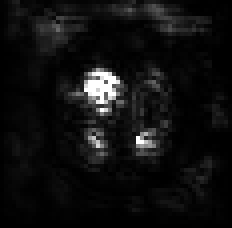
\includegraphics[width=\linewidth]{Images/AnPe/10771_guided} &
		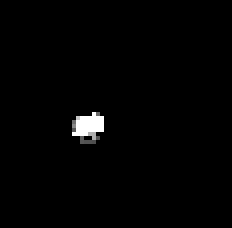
\includegraphics[width=\linewidth]{Images/AnPe/10771_vanil}\\ 
		5.1a Ursprungsbild &5.1b Guided Backprop. &5.1c Vanilla Saliency \\
		Höchstgeschwindigkeit (30) & Überholverbot & Höchstgeschwindigkeit (30)\\
		& 0.9155 & 0.9283\\
		
	\end{tabular} 

	\caption{Ergebnisse von verschiedenen Verfahren am selben Bild. }
	\label{tab:sal1}
\end{table}


Tabelle \ref{tab:sal1} zeigt exemplarisch, wie aus dem Ursprungsbild (5.1a „Höchstgeschwindigkeit (30)“), unter Verwendung des „Smoothed Guided Backpropagation“ Verfahrens, ein Bild erzeugt wurde, das vom Black Box Modell mit 91,55\% als „Überholverbot“ klassifiziert wurde (5.1b). 
Das „Smoothed Vanilla Saliency“ Verfahren erzeugte hingegen aus demselben Ursprungsbild ein Bild, das mit einer Zielkonfidenz von 92,83\% vom Black Box Modell als „Höchstgeschwindigkeit (30)“ erkannt wurde (5.1c).
%\begin{figure}
%	\begin{subfigure}{.33\textwidth}
%		\centering
%		
\includegraphics[width=.8\linewidth]{Images/AnPe/10771}
%		\caption{Ursprungsbild (Höchstgeschwindigkeit 30)}
%		\label{fig:ursprung1}
%	\end{subfigure}%penis
%	\begin{subfigure}{.33\textwidth}
%		\centering
%		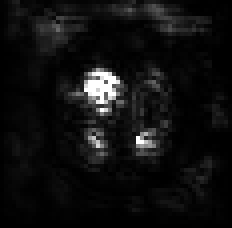
\includegraphics[width=.8\linewidth]{Images/AnPe/10771_guided}
%		\caption{Halblabor.}
%		\label{fig:salmap1}
%	\end{subfigure}
%	\begin{subfigure}{.33\textwidth}
%		\centering
%		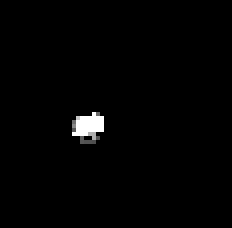
\includegraphics[width=.8\linewidth]{Images/AnPe/10771_vanil}
%		\caption{Freie Umgebung.}
%		\label{fig:salmap_1}
%	\end{subfigure}
%\end{figure}

Tabelle \ref{tab:sal2} veranschaulicht weitere Beispiele für erfolgreich erzeugte Bilder, unter Verwendung der optimierten Saliency Map Verfahren. Wieder kann beobachtet werden, dass die erzeugten Bilder zwar mit einer Zielkonfidenz von mehr als 90\% vom Black Box Modell klassifiziert wurden, die ursprüngliche Klasse jedoch abweicht.

\begin{table}
	\centering
	\begin{tabular}{p{4.5cm}p{4.5cm}}
		
\includegraphics[height=4.4cm]{Images/AnPe/11240} &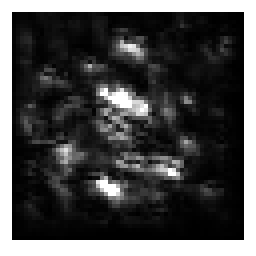
\includegraphics[width=\linewidth]{Images/AnPe/11240_guided}  \\
		& Guided Backprop.\\
		Rechts Vorbei & Einmalige Vorfahrt\\
		& 0.9678\\
		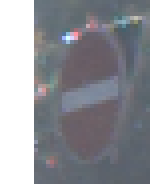
\includegraphics[height=4.4cm]{Images/AnPe/06848} &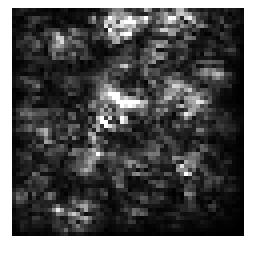
\includegraphics[width=\linewidth]{Images/AnPe/06848_s_int}  \\
		& Integrated Grad.\\
		Einfahrt Verboten & Überholverbot\\
		& 0.9571\\
		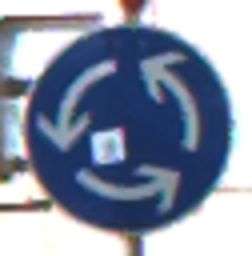
\includegraphics[height=4.4cm]{Images/AnPe/04709} &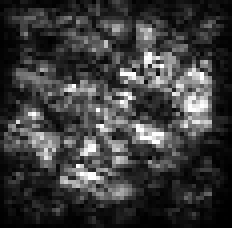
\includegraphics[width=\linewidth]{Images/AnPe/04709_int_grad}  \\
		& Integrated Grad.\\
		Kreisverkehr &Baustelle \\
		& 0.9999
	\end{tabular}
	\caption{Weitere Beispiele für Irrbilder mit Konfidenz >0.9 inklusive entsprechendem Ursprungsbild und verwendetem Verfahren.}
\label{tab:sal2}
\end{table}


Zusammenfassend konnte hiermit gezeigt werden, dass die in Kapitel 5.1 formulierten Hypothesen zutreffen und sich Bilder – unter Verwendung eines eigens trainierten \ac{CNN} Modells („Aphrodite“) sowie verschiedener Saliency Map Verfahren – erzeugen lassen, die zwar keine für den Menschen sinnvolle Bedeutung haben, jedoch beim Black Box Modell Zielkonfidenzen von mehr als 90\% erreichten.


%Zusammenfassend konnte gezeigt werden, dass es mithilfe der Erstellung von Saliency Maps an einem eigenen Modell Bilder erzeugt werden können, welche von einem unbekanntem \ac{NN} mit hohen Konfidenzen verschiedenen Klassen zugeordnet werden. Die Erfolgsrate in Relation zur Anzahl erzeugter Bilder und dem Rechenaufwand ist dabei jedoch gering und es herrscht aktuell keine verlässliche Aussagekraft darüber, welcher Klasse das erzeugte Bild zugeordnet wird. 

\chapter{Gradient Ascent}
\label{cha:gascent}

Beim Training von künstlichen neuronalen Netzwerken, wie etwa \ac{CNN}, werden die Gewichte $ w_{i} $ und der Schwellwerte (Bias) so lange verändert und im Modell des Netzwerks gespeichert, bis die Ausgabe aus dem Netzwerk die Eingabedaten (Trainingsbilder) annähern. 
Um zu quantifizieren, wie gut dieses Ziel erreicht wird, wird eine sogenannte Kostenfunktion (engl. cost function) definiert. 
Die Kostenfunktion geht also über jedes einzelne Bild aus dem Trainingsdatensatz und berechnet den Unterschied zwischen der gewünschten Ausgabe und dem Ausgabevektor $\vec{a}$ des Netzwerks.
Der Ausgabevektor $\vec{a}$ ist hierbei abhängig vom Eingabebild, dem Gewicht $w_{i}$ und dem Schwellwert.
Die Kostenfunktion hat den Wert 0 in etwa dann angenähert, wenn das Eingabebild annähernd dem Ausgabevektor $\vec{a}$ entspricht, was das Ziel des Trainings eines künstlichen neuronalen Netzwerks darstellt. Denn dann wurde das Eingabebild korrekt erkannt.
Im Rahmen des Trainings sollen also eine Reihe von Gewichten $w_{i}$ und Schwellwerten gefunden werden, welche zu einer minimalen Kostenfunktion führen. 
Dies wird erreicht mit dem Gradient Descent-Algorithmus\cite{zhou_understanding_2018}.
Dieser Algorithmus berechnet wiederholt den Gradienten und verbessert iterativ die Gewichte. 


Das \textit{Gradient Ascent}-Verfahren ist als Pendant zum Gradient Descent-Verfahren zu verstehen. Hier wird auf die berechneten Gradienten eines trainierten Convolutional Neural Networks zugegriffen und das Eingabebild so lange verändert, bis dies dem gewünschten Ergebnisbild entspricht.
\section{Konzept}
Um gegebene \ac{CNN} gezielt anzugreifen, das heißt Bilder zu erzeugen, die einer bestimmten Zielklasse entsprechen und gleichzeitig vom Menschen nicht als solche erkannt werden, eignet sich die Methode \textit{Targeted Backpropagation}, welche eine Variante des \textit{Gradient Ascent}-Verfahrens darstellt \cite{liu_delving_2016}.
Diese Methode setzt ein bereits trainiertes \ac{CNN} voraus, greift auf die Gradienten des Modells zu und verändert das Eingabebild – wie etwa ein zufallsgeneriertes Bild – so lange, bis es der gewünschten Zielklasse entspricht oder diese annähert. 
Bei diesem Verfahren kann man beobachten, dass relevante Pixel, welche die bedeutendsten Stellen im Bild repräsentieren, stärker mutiert werden als unwichtige Pixel, die weitgehend unverändert bleiben.
\section{Implementierung}

Zunächst wird als vorverarbeitender Schritt ein \ac{CNN} unter Verwendung der AlexNet Architektur in PyTorch trainiert. 
Die hierbei verwendete Architektur des AlexNet entstammt \cite{pytorch_datasets_2019} und wurde dahingehend modifiziert, dass das AlexNet zu Eingabebildern der Größe $64 \times 64$ Pixel, drei Farbkanälen (RGB) sowie zu den 43 Klassen aus dem \ac{GTSRB} Datensatz kompatibel ist. 
Die Bilder aus dem \ac{GTSRB} Trainingsdatensatz, welche unterschiedliche Bildgrößen aufweisen, wurden im Zuge des Trainings ebenfalls auf eine Bildgröße von 64 x 64 Pixel interpoliert. 
Das Training des AlexNet erfolgte 50 Epochen lang mit dem \ac{GTSRB} Trainingsdatensatz und erzielte mit dem \ac{SGD}-Optimierer eine Genauigkeit von annähernd 89\% (validiert mit dem \ac{GTSRB} Testdatensatz).
Die Implementierung des \textit{Gradient Ascent}-Verfahrens, unter Verwendung der \textit{Targeted Backpropagation}-Methode und dem trainierten AlexNet, erfolgte in einer modifizierten Variante zu \cite{ozbulak_pytorch_2019}. 

Unter Angabe der Zielklasse sowie der minimalen Zielkonfidenz erzeugt der Algorithmus zunächst ein Zufallsbild, welches als Eingabeparameter für das trainierte AlexNet verwendet wird. Unter Anwendung des SGD-Optimierers auf das Eingabebild werden die Gradienten entsprechend der spezifizierten Zielklasse berechnet. 

Diese Gradienten werden nicht verwendet, um die Parameter des AlexNet-Mo"-dells zu verändern, wie es beim Training der Fall war, sondern um das eingegebene Bild dahingehend zu modifizieren, dass es der gewünschten Zielklasse entspricht. 
Die entsprechenden Pixel der aktivierten Neuronen werden hierzu (je nach Aktivierungsstärke) mit den Bildpixelwerten addiert. 
Dieser Prozess wird so lange wiederholt, bis das veränderte Bild die gewünschte Konfidenz zu der angegebenen Zielklasse erreicht hat.

Der Algorithmus wurde für jede der 43 \ac{GTSRB}-Klassen so lange wiederholt, bis das veränderte Bild die gewünschte Mindest-Konfidenz von 100\% erreicht.
Zur abschließenden Evaluierung der erzeugten Bilder am \ac{NN} des \ac{GI}-Wettbewerbs, werden alle Bilder an das Webinterface des Wettbewerbs gesendet. Die Informationen, das heißt die vom \ac{NN} des \ac{GI}-Wettbewerbs erkannte Zielklasse und Konfidenz, werden anschließend aus dem HTTP-Responsecode zu jedem übermittelten Bild in zwei verschiedenen Logdateien gespeichert: Die erste Logdatei speichert alle Ergebnisse aus dem jeweiligen HTTP-Responsecode, wohingegen die zweite Logdatei nur gefilterte Ergebnisse, das heißt Konfidenzen von mehr als 90\%, zu den übermittelten Bildern enthält.


\section{Ergebnisse}
Mit dem \textit{Gradient Ascent}-Verfahren, unter Verwendung der \textit{Targeted Backpropagation}-Methode, wurden 43 Farbbilder – also je ein Bild zu jeder \ac{GTSRB}-Klasse – erzeugt. 
Die erzeugten Bilder sind hierbei vom Menschen nicht als Verkehrszeichen wahrnehmbar. 
Jedoch klassifizierte das \ac{NN} des \ac{GI}-Wettbewerbs nur 20 der 43 erzeugten Bilder mit einer Konfidenz von über 90\% als Verkehrszeichen. 

Unter diesen 20 erzeugten Bildern stimmte lediglich bei 10 Bildern die im Algorithmus angegebene Zielklasse mit der vom \ac{NN} des \ac{GI}-Wettbewerbs ausgegebenen Klasse überein.

Tabelle \ref{tab:gasc1} veranschaulicht vier repräsentative Ergebnisse, welche mit dem \textit{Gradient Ascent}-Verfahren erzeugt und vom \ac{NN} des \ac{GI}-Wettbewerbs mit einer Konfidenz von über 90\% als Verkehrszeichen klassifiziert werden.
Die Abbildungen oben links und unten rechts wurden vom \ac{NN} des \ac{GI}-Wettbewerbs als "`Einfahrt Verboten"' mit 99,99\% Konfidenz beziehungsweise als "`Kreisverkehr"' mit 98,68\% Konfidenz korrekt klassifiziert. 
Das heißt, die im Algorithmus angegebene Zielklasse entsprechen der tatsächlichen Zielklasse.
Hingegen weicht bei den beiden anderen Bildern (oben rechts und unten links) die im Algorithmus angegebene Zielklasse von der tatsächlich erkannten Zielklasse ab. 
Bei Abbildung oben rechts wird im Algorithmus "`Ausschließlich links"' als Zielklasse angegeben. 
Das erzeugte Bild wird mit einer Konfidenz von 95,35\% vom \ac{NN} des \ac{GI}-Wettbewerbs als "`Kreisverkehr"' erkannt.
Bei Abbildung unten links wird im Algorithmus "`Links vorbei"' als Zielklasse angegeben. 
Das erzeugte Bild wird mit einer Konfidenz von 99,50\% als "`Rechts vorbei"' vom \ac{NN} des \ac{GI}-Wettbewerbs erkannt.


\begin{table}
	\centering
\begin{tabular}{p{4.4cm}p{4.4cm}}
	\centering
	
\includegraphics[width=\linewidth]{Images/AnPe/17_Einfahrtverbot} &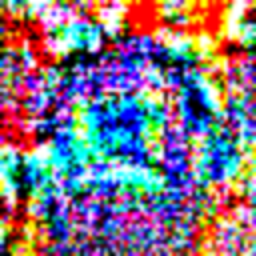
\includegraphics[width=\linewidth]{Images/AnPe/34_kreisverkehr_origTurnleft}  \\
	6.1a: Einfahrt verboten & 6.1b: Kreisverkehr \\
	99,99\% Konfidenz&95,35\% Konfidenz\\
	
\includegraphics[width=\linewidth]{Images/AnPe/39_RechtsVorbeiOrigLinksvorbei} &
\includegraphics[width=\linewidth]{Images/AnPe/40_kreisverkehr}  \\
	6.1c: Rechts Vorbei&6.1d: Kreisverkehr\\
	99,50\% Konfidenz&98,68\% Konfidenz\\
\end{tabular}

\caption{Ergebnisse mit dem \textit{Gradient Ascent}-Verfahren (\textit{Targeted Backpropagation})}
\label{tab:gasc1}
\end{table}


\chapter{Fazit}
\label{cha:Fazit} \label{cha:Schluss}
Nach einer abschließenden Zusammenfassung, werden in diesem Kapitel zusätzlich die verschiedenen Ansätze verglichen und bewertet. Aus dieser Diskussion werden die Einschränkungen und Möglichkeiten für weitere Arbeiten angesprochen.

\section{Zusammenfassung} ~\newline 
\todo{Ergebnisse Degen}

Desweiteren konnten Erfolge mit der Erzeugung von Saliency Maps in den geglätteten Varianten verbucht werden. Somit konnte bestätigt werden, dass die Visualisierung der Relevanten Pixel für ein Bild mit hoher Konfidenz geeignet sind, um als "minimale Beispiele" für das NN verwendet werden können. Die entsprechenden Verfahren erzeugten Täuschungen mit Konfidenzen >0.9, allerdings lassen sich keine Aussagen über die allgemeine Verlässlichkeit und Zielgerichtetheit treffen.

Zuletzt konnte auch mit dem \textit{Gradient Ascent} Verfahren sehr gute ergebnisse erzielt werden. für 10 von 43 Klassen konnten Täuschungen mit hohen Konfidenzen am Remote-NN erzielt werden. Es wird vermutet dass die Ausbeute mit weiterer Optimierung vergrößert werden kann oder auch echte Bilder für die Erzeugung der Täuschungen verwendet werden können.



\section{Diskussion}
Die Herausforderungen des Wettbewerbs wirken sich auf die Erfolge der Verfahren aus. Es wird vermutet das beide Verfahren \textit{Saliency Map} und \textit{Gradient Ascent} bessere ergebnisse liefern Könnten, wenn das verwendete Bild größer als $64\times64$ wäre. Desweiteren kann nichts über die Validierungsgenauigkeit des Trasi-NN gesagt werden, weshalb auch die nicht zielgerichteten Täuschungsbilder als gutes Ergebnis betitelt werden. 


Im Vergleich der Methoden \textit{Saliency Map} und \textit{Gradient Ascent}, kann das letztere bevorzugt werden. 



hier kommen rein
vergleich der ergebnisse (reproduzierbarkeit, gezielt/random, qualität der bilder)
- einschränkungen probleme unserer ansätze, 


wichtig: eigene fehler oder einschränkungen der methodik erkennen.



\section{Weiterführende Arbeiten}~\newline 
Die Ergebnisse dieser Arbeit liefern weitere Ansätze für zukünftige Aufgaben. Zum einen können die verwendeten Ansätze individuell weiter Optimiert werden, bezüglich des selbsterstellten lokalen Neuronalem Netz und der Algorithmik bzw. deren Parameter. Desweiteren können verfahren entwickelt werden, die sich aller Methoden gezielt bedienen. 
%content
%Vergleich mit einem Framework, wie zum Beispiel CleverHans \footnote, Vergleich von einem gut und schlecht trainierten Modell, wie arg unterscheiden sich daraus generierte Bilder (lohnt es sich), wie wichtig ist die Bildgröße, 
\newpage\newpage

% ---------------------------- Literaturverzeichnis ----------------------------------------------
\bibliographystyle{plain}
\bibliography{src}


% ------------------------------- Anhang ---------------------------------------------------------

\begin{appendix}
\clearpage
\pagenumbering{Roman}						% römische Seitenzahlen für Anhang
\chapter{Anhang}
\section*{Aphrodite Summary}
\label{app:Aphrodite}
\begin{figure}[h]
	\centering
	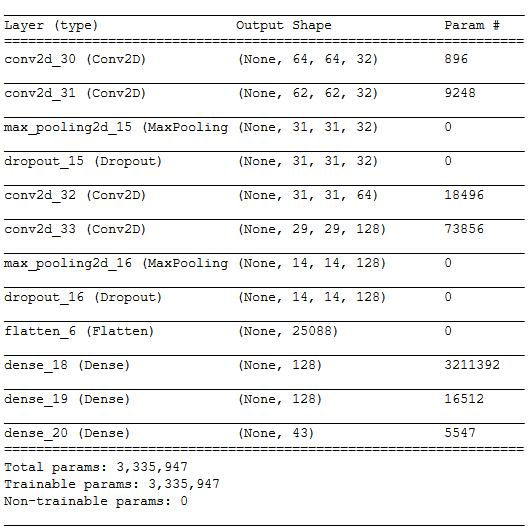
\includegraphics[width=0.9\linewidth]{Images/AphroditeSummary}
	\label{fig:aphroditesummary}
\end{figure}

\end{appendix}


\end{document}
